\documentclass{standalone}
\usepackage{tikz}
\usetikzlibrary{patterns, positioning}

\begin{document}
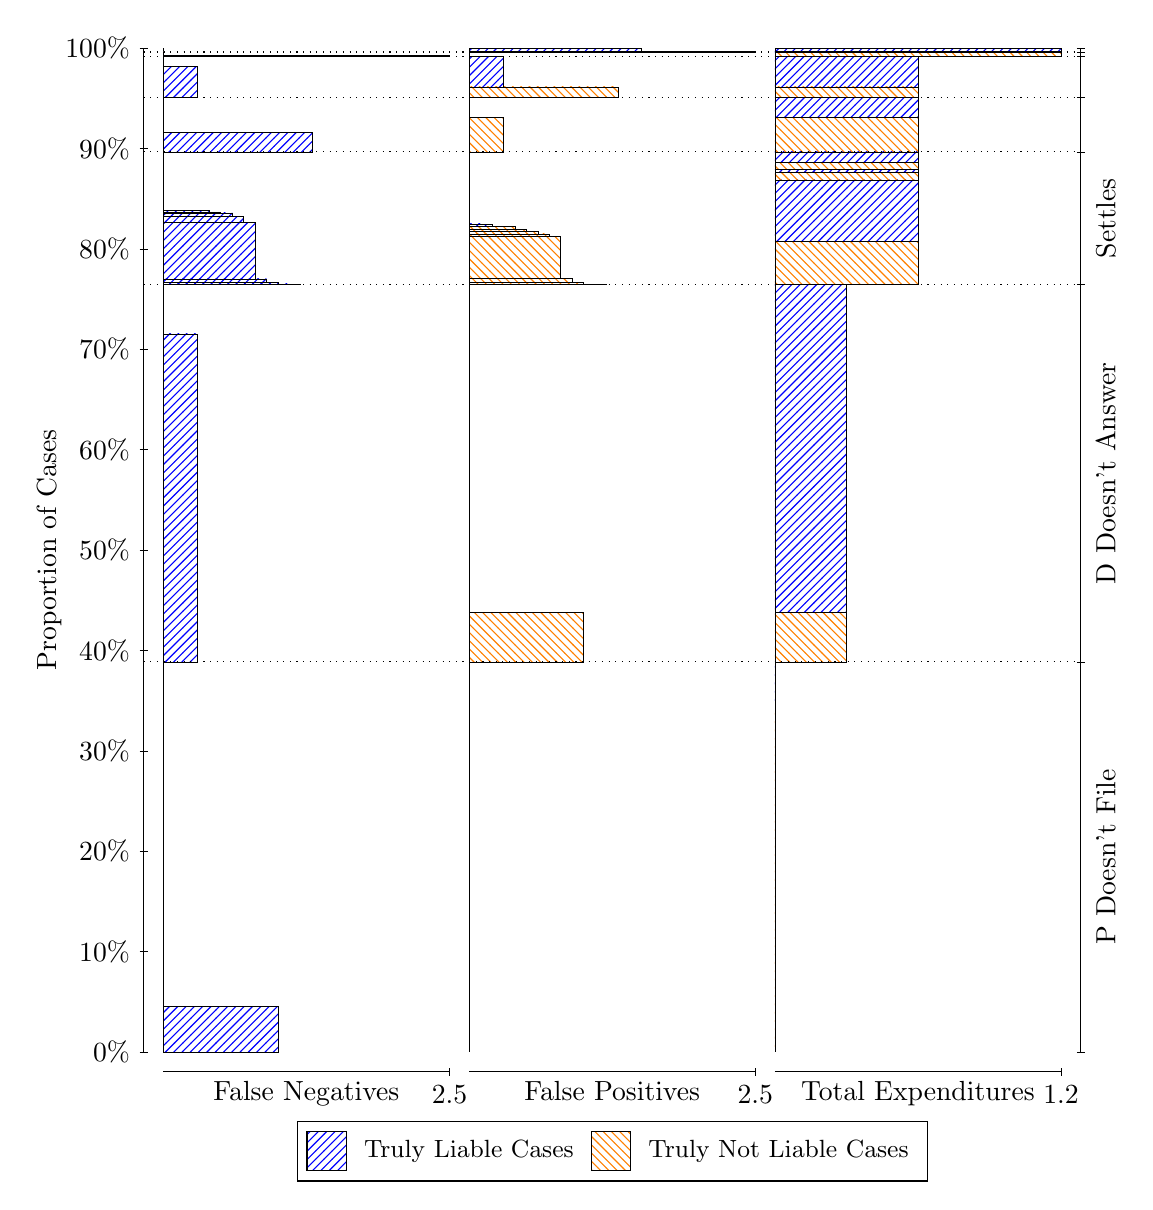
\begin{tikzpicture}
\draw[black, very thin] (1.5,1.75) -- (1.5,14.5);
\node[rotate=90, anchor=center] at (0.3, 8.125) {Proportion of Cases};
\draw[black, very thin] (1.45,1.75) -- (1.55,1.75);
\node[anchor=east] at (1.45, 1.75) {0\%};
\draw[black, very thin] (1.45,3.025) -- (1.55,3.025);
\node[anchor=east] at (1.45, 3.025) {10\%};
\draw[black, very thin] (1.45,4.3) -- (1.55,4.3);
\node[anchor=east] at (1.45, 4.3) {20\%};
\draw[black, very thin] (1.45,5.575) -- (1.55,5.575);
\node[anchor=east] at (1.45, 5.575) {30\%};
\draw[black, very thin] (1.45,6.85) -- (1.55,6.85);
\node[anchor=east] at (1.45, 6.85) {40\%};
\draw[black, very thin] (1.45,8.125) -- (1.55,8.125);
\node[anchor=east] at (1.45, 8.125) {50\%};
\draw[black, very thin] (1.45,9.4) -- (1.55,9.4);
\node[anchor=east] at (1.45, 9.4) {60\%};
\draw[black, very thin] (1.45,10.675) -- (1.55,10.675);
\node[anchor=east] at (1.45, 10.675) {70\%};
\draw[black, very thin] (1.45,11.95) -- (1.55,11.95);
\node[anchor=east] at (1.45, 11.95) {80\%};
\draw[black, very thin] (1.45,13.225) -- (1.55,13.225);
\node[anchor=east] at (1.45, 13.225) {90\%};
\draw[black, very thin] (1.45,14.5) -- (1.55,14.5);
\node[anchor=east] at (1.45, 14.5) {100\%};

\draw[black, very thin] (13.4,1.75) -- (13.4,14.5);
\draw[black, very thin] (13.35,1.75) -- (13.45,1.75);
\node[anchor=west] at (13.35, 1.75) {};
\draw[black, very thin] (13.35,6.7044) -- (13.45,6.7044);
\node[anchor=west] at (13.35, 6.7044) {};
\draw[black, very thin] (13.35,11.495) -- (13.45,11.495);
\node[anchor=west] at (13.35, 11.495) {};
\draw[black, very thin] (13.35,13.181) -- (13.45,13.181);
\node[anchor=west] at (13.35, 13.181) {};
\draw[black, very thin] (13.35,13.875) -- (13.45,13.875);
\node[anchor=west] at (13.35, 13.875) {};
\draw[black, very thin] (13.35,14.395) -- (13.45,14.395);
\node[anchor=west] at (13.35, 14.395) {};
\draw[black, very thin] (13.35,14.45) -- (13.45,14.45);
\node[anchor=west] at (13.35, 14.45) {};
\draw[black, very thin] (13.35,14.5) -- (13.45,14.5);
\node[anchor=west] at (13.35, 14.5) {};

\draw[black, very thin, pattern color=blue, pattern=north east lines] (1.75,1.75) rectangle (3.2033,2.3257);
\draw[black, very thin, pattern color=orange, pattern=north west lines] (1.75,2.3257) rectangle (1.75,6.7044);
\draw[black, very thin, pattern color=blue, pattern=north east lines] (1.75,6.7044) rectangle (2.186,10.87);
\draw[black, very thin, pattern color=orange, pattern=north west lines] (1.75,10.87) rectangle (1.75,11.495);
\draw[black, very thin, pattern color=blue, pattern=north east lines] (1.75,11.495) rectangle (3.494,11.502);
\draw[black, very thin, pattern color=blue, pattern=north east lines] (1.75,11.502) rectangle (3.3487,11.506);
\draw[black, very thin, pattern color=blue, pattern=north east lines] (1.75,11.506) rectangle (3.2033,11.523);
\draw[black, very thin, pattern color=blue, pattern=north east lines] (1.75,11.523) rectangle (3.058,11.524);
\draw[black, very thin, pattern color=blue, pattern=north east lines] (1.75,11.524) rectangle (3.058,11.569);
\draw[black, very thin, pattern color=blue, pattern=north east lines] (1.75,11.569) rectangle (2.9127,12.285);
\draw[black, very thin, pattern color=blue, pattern=north east lines] (1.75,12.285) rectangle (2.7673,12.358);
\draw[black, very thin, pattern color=blue, pattern=north east lines] (1.75,12.358) rectangle (2.622,12.407);
\draw[black, very thin, pattern color=blue, pattern=north east lines] (1.75,12.407) rectangle (2.4767,12.417);
\draw[black, very thin, pattern color=blue, pattern=north east lines] (1.75,12.417) rectangle (2.3313,12.437);
\draw[black, very thin, pattern color=orange, pattern=north west lines] (1.75,12.437) rectangle (1.75,13.181);
\draw[black, very thin, pattern color=blue, pattern=north east lines] (1.75,13.181) rectangle (3.6393,13.431);
\draw[black, very thin, pattern color=orange, pattern=north west lines] (1.75,13.431) rectangle (1.75,13.875);
\draw[black, very thin, pattern color=blue, pattern=north east lines] (1.75,13.875) rectangle (2.186,14.264);
\draw[black, very thin, pattern color=orange, pattern=north west lines] (1.75,14.264) rectangle (1.75,14.395);
\draw[black, very thin, pattern color=blue, pattern=north east lines] (1.75,14.395) rectangle (5.3833,14.405);
\draw[black, very thin, pattern color=orange, pattern=north west lines] (1.75,14.405) rectangle (1.75,14.45);
\draw[black, very thin, pattern color=orange, pattern=north west lines] (1.75,14.45) rectangle (1.75,14.458);
\draw[black, very thin, pattern color=blue, pattern=north east lines] (1.75,14.458) rectangle (1.75,14.5);
\draw[black, very thin, pattern color=orange, pattern=north west lines] (5.6333,1.75) rectangle (5.6333,6.1286);
\draw[black, very thin, pattern color=blue, pattern=north east lines] (5.6333,6.1286) rectangle (5.6333,6.7044);
\draw[black, very thin, pattern color=orange, pattern=north west lines] (5.6333,6.7044) rectangle (7.0867,7.3294);
\draw[black, very thin, pattern color=blue, pattern=north east lines] (5.6333,7.3294) rectangle (5.6333,11.495);
\draw[black, very thin, pattern color=orange, pattern=north west lines] (5.6333,11.495) rectangle (7.3773,11.498);
\draw[black, very thin, pattern color=orange, pattern=north west lines] (5.6333,11.498) rectangle (7.232,11.501);
\draw[black, very thin, pattern color=orange, pattern=north west lines] (5.6333,11.501) rectangle (7.0867,11.527);
\draw[black, very thin, pattern color=orange, pattern=north west lines] (5.6333,11.527) rectangle (6.9413,11.578);
\draw[black, very thin, pattern color=orange, pattern=north west lines] (5.6333,11.578) rectangle (6.796,12.103);
\draw[black, very thin, pattern color=orange, pattern=north west lines] (5.6333,12.103) rectangle (6.6507,12.139);
\draw[black, very thin, pattern color=orange, pattern=north west lines] (5.6333,12.139) rectangle (6.5053,12.171);
\draw[black, very thin, pattern color=orange, pattern=north west lines] (5.6333,12.171) rectangle (6.36,12.193);
\draw[black, very thin, pattern color=orange, pattern=north west lines] (5.6333,12.193) rectangle (6.2147,12.238);
\draw[black, very thin, pattern color=blue, pattern=north east lines] (5.6333,12.238) rectangle (5.924,12.258);
\draw[black, very thin, pattern color=blue, pattern=north east lines] (5.6333,12.258) rectangle (5.7787,12.268);
\draw[black, very thin, pattern color=blue, pattern=north east lines] (5.6333,12.268) rectangle (5.6333,13.181);
\draw[black, very thin, pattern color=orange, pattern=north west lines] (5.6333,13.181) rectangle (6.0693,13.624);
\draw[black, very thin, pattern color=blue, pattern=north east lines] (5.6333,13.624) rectangle (5.6333,13.875);
\draw[black, very thin, pattern color=orange, pattern=north west lines] (5.6333,13.875) rectangle (7.5227,14.006);
\draw[black, very thin, pattern color=blue, pattern=north east lines] (5.6333,14.006) rectangle (6.0693,14.395);
\draw[black, very thin, pattern color=orange, pattern=north west lines] (5.6333,14.395) rectangle (5.6333,14.44);
\draw[black, very thin, pattern color=blue, pattern=north east lines] (5.6333,14.44) rectangle (5.6333,14.45);
\draw[black, very thin, pattern color=orange, pattern=north west lines] (5.6333,14.45) rectangle (9.2667,14.458);
\draw[black, very thin, pattern color=blue, pattern=north east lines] (5.6333,14.458) rectangle (7.8133,14.5);
\draw[black, very thin, pattern color=orange, pattern=north west lines] (9.5167,1.75) rectangle (9.5167,6.1286);
\draw[black, very thin, pattern color=blue, pattern=north east lines] (9.5167,6.1286) rectangle (9.5167,6.7044);
\draw[black, very thin, pattern color=orange, pattern=north west lines] (9.5167,6.7044) rectangle (10.425,7.3294);
\draw[black, very thin, pattern color=blue, pattern=north east lines] (9.5167,7.3294) rectangle (10.425,11.495);
\draw[black, very thin, pattern color=orange, pattern=north west lines] (9.5167,11.495) rectangle (11.333,12.049);
\draw[black, very thin, pattern color=blue, pattern=north east lines] (9.5167,12.049) rectangle (11.333,12.825);
\draw[black, very thin, pattern color=orange, pattern=north west lines] (9.5167,12.825) rectangle (11.333,12.926);
\draw[black, very thin, pattern color=blue, pattern=north east lines] (9.5167,12.926) rectangle (11.333,12.955);
\draw[black, very thin, pattern color=orange, pattern=north west lines] (9.5167,12.955) rectangle (11.333,13.043);
\draw[black, very thin, pattern color=blue, pattern=north east lines] (9.5167,13.043) rectangle (11.333,13.181);
\draw[black, very thin, pattern color=orange, pattern=north west lines] (9.5167,13.181) rectangle (11.333,13.624);
\draw[black, very thin, pattern color=blue, pattern=north east lines] (9.5167,13.624) rectangle (11.333,13.875);
\draw[black, very thin, pattern color=orange, pattern=north west lines] (9.5167,13.875) rectangle (11.333,14.006);
\draw[black, very thin, pattern color=blue, pattern=north east lines] (9.5167,14.006) rectangle (11.333,14.395);
\draw[black, very thin, pattern color=orange, pattern=north west lines] (9.5167,14.395) rectangle (13.15,14.44);
\draw[black, very thin, pattern color=blue, pattern=north east lines] (9.5167,14.44) rectangle (13.15,14.45);
\draw[black, very thin, pattern color=orange, pattern=north west lines] (9.5167,14.45) rectangle (13.15,14.458);
\draw[black, very thin, pattern color=blue, pattern=north east lines] (9.5167,14.458) rectangle (13.15,14.5);
\draw[black, dotted] (1.5,6.7044) -- (13.4,6.7044);
\draw[black, dotted] (1.5,11.495) -- (13.4,11.495);
\draw[black, dotted] (1.5,13.181) -- (13.4,13.181);
\draw[black, dotted] (1.5,13.875) -- (13.4,13.875);
\draw[black, dotted] (1.5,14.395) -- (13.4,14.395);
\draw[black, dotted] (1.5,14.45) -- (13.4,14.45);
\draw[black, very thin] (1.75,1.5) -- (5.3833,1.5);
\node[anchor=north] at (3.5667, 1.5) {False Negatives};
\draw[black, very thin] (5.3833,1.45) -- (5.3833,1.55);
\node[anchor=north] at (5.3833, 1.45) {2.5};

\draw[black, very thin] (5.6333,1.5) -- (9.2667,1.5);
\node[anchor=north] at (7.45, 1.5) {False Positives};
\draw[black, very thin] (9.2667,1.45) -- (9.2667,1.55);
\node[anchor=north] at (9.2667, 1.45) {2.5};

\draw[black, very thin] (9.5167,1.5) -- (13.15,1.5);
\node[anchor=north] at (11.333, 1.5) {Total Expenditures};
\draw[black, very thin] (13.15,1.45) -- (13.15,1.55);
\node[anchor=north] at (13.15, 1.45) {1.2};

\node[black, centered, rotate=90] at (13.72, 4.2272) {P Doesn't File};
\node[black, centered, rotate=90] at (13.72, 9.0995) {D Doesn't Answer};
\node[black, centered, rotate=90] at (13.72, 12.338) {Settles};





\draw (7.449999999999999,1.5) node[draw=none] (baseCoordinate) {};
\begin{scope}[align=center]
        \matrix[scale=0.5, draw=black, below=0.5cm of baseCoordinate, nodes={draw}, column sep=0.1cm]{
            \node[rectangle, draw, minimum width=0.5cm, minimum height=0.5cm, pattern=north east lines, pattern color=blue] {}; &
            \node[draw=none, font=\small] (B) {Truly Liable Cases}; &
            \node[rectangle, draw, minimum width=0.5cm, minimum height=0.5cm, pattern=north west lines, pattern color=orange] {}; &
            \node[draw=none, font=\small] (B) {Truly Not Liable Cases}; \\
            };
\end{scope}

\end{tikzpicture}
\end{document}